\documentclass{beamer}
\usepackage{beamerthemeCVC}
\usepackage{graphicx}

\usepackage{xmpmulti}

%% PRESENTATION CONFIGURATION PARAMETERS %%%%%%%%%%%%%%%%%%%%%%%%%%%%%%%%%%%%%%%
\titlebackgroundfile{images/template_title}
%\framebackgroundfile{images/template_frame}
\framebackgroundfile{images/template_frame_v01}
%\definecolor{vermell}{HTML}{8C2423}
\definecolor{vermell}{HTML}{000066}
\definecolor{gris}{HTML}{4C4C4C}

\usefonttheme{structurebold}

\setbeamercolor{author in head/foot}{fg=white}
\setbeamercolor{title in head/foot}{fg=white}
\setbeamercolor{section in head/foot}{fg=vermell}
\setbeamercolor{normal text}{fg=gris}
\setbeamercolor{frametitle}{fg=vermell}
%\setbeamercolor{frametitle}{fg=blue!20!black}
\setbeamerfont{block title}{size={}}
\setbeamerfont{author}{size=\footnotesize}
\setbeamerfont{date}{size=\footnotesize}
\setbeamertemplate{itemize item}[circle]
\setbeamertemplate{itemize subitem}[circle]
\setbeamertemplate{itemize subsubitem}[circle]
\setbeamertemplate{itemize subsubsubitem}[circle]
\setbeamercolor{itemize item}{fg=vermell}
\setbeamercolor{itemize subitem}{fg=vermell}
\setbeamercolor{itemize subsubitem}{fg=vermell}
\setbeamercolor{itemize subsubsubitem}{fg=vermell}
\setbeamercolor{enumerate item}{fg=vermell}
\setbeamercolor{enumerate subitem}{fg=vermell}
\setbeamercolor{enumerate subsubitem}{fg=vermell}
\setbeamercolor{enumerate subsubsubitem}{fg=vermell}
\setbeamercolor{alerted text}{fg=vermell}
\setbeamerfont{alerted text}{series=\bfseries}
% This command makes that acrobat reader doesn't changes the colors of the slide
% when there are figures with transparencies.
\pdfpageattr {/Group << /S /Transparency /I true /CS /DeviceRGB>>}




\graphicspath{{images/}}



%%%%%%%%%%%%%%%%%%%%%%%%%%%%%%%%%%%%%%%%%%%%%%%%%%%%%%%%%%%%%%%%%%%%%%%%%%%%%%%%

%      + Short title.               + Title which appears in the cover.
%      v                            v
%\title[Beamer presentation example]{Nonlinear Dynamics Approach to Human Activity Recognition Using Inertial Sensors}
\vspace{5mm}
\title[Time-delay Embedding Example]
{Time-delay Embedding Example}
%       + Short author names which appear in the slides.
%       v
\author[Miguel P. Xochicale]
{   % Author names which appear in the cover page.
    %Perez-Xochicale Miguel Angel\inst{1}
    \textbf{Miguel P. Xochicale }
}
%          + Short affiliation which appears in the slides.
%          v
\institute[CVC-IIIA]
{   % Affiliation information which appears in the cover page.

      \vspace{5mm}
    \begin{tabular}{c}
    %\inst{1}Internal Research Conference 
    \end{tabular}
}
%     + Short acronym of the conference or date of the presentation.
%     v
\date[DEMO-2013]
{   % Conference name which appears in the cover page.
          18-21 October 2016
}





\begin{document}
% Creates the cover page.
\frame{\titlepage}


%+++++++++++++++++++++++++++++++++++++++++++++++++++
%+++++++++++++++++++++++++++++++++++++++++++++++++++
\section{State Space Representation}


%+++++++++++++++++++++++++++++++++++++++++++++++++++
\begin{frame}
\frametitle{Reconstructed State Space}
\vspace{-5mm}

\begin{figure}
\centering 
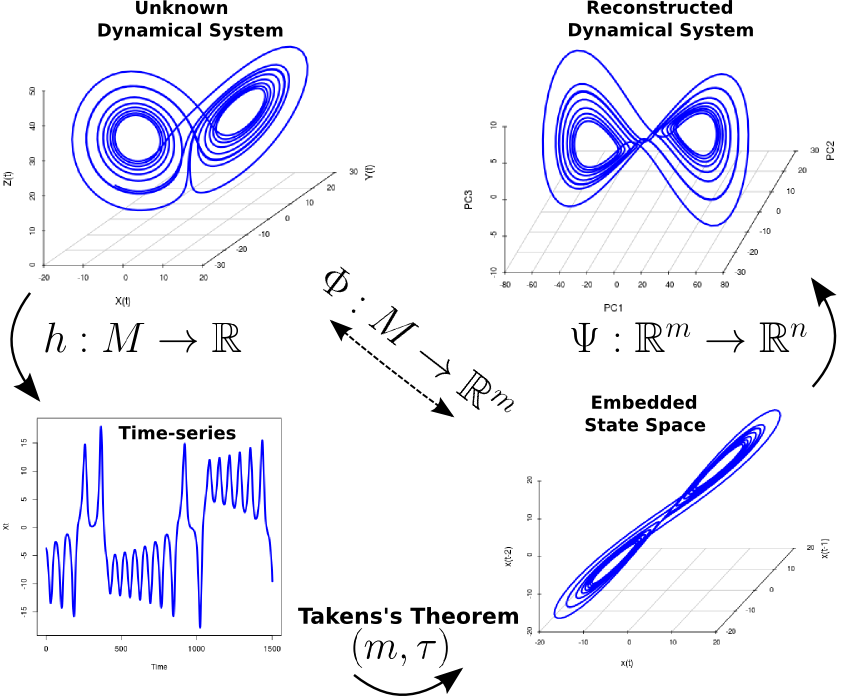
\includegraphics[scale=.35]{takens_theorem_v5} 
\end{figure}

\end{frame}
%---------------------------------------------------






%+++++++++++++++++++++++++++++++++++++++++++++++++++
 \begin{frame}
 \frametitle{Time-Delay Embedding Example }
   
  \begin{columns}[onlytextwidth]
    \begin{column}{0.3\textwidth}
Lorenz System
 \begin{eqnarray*} 
  \frac{dx}{dt} &=&\sigma (x-y), \\
  \frac{dx}{dt} &=&x (\rho -z) - y, \\ 
  \frac{dx}{dt} &=&xy - \beta z.
 \end{eqnarray*}
 \end{column} 
  
  \begin{column}{0.63\textwidth}
       \begin{figure}
 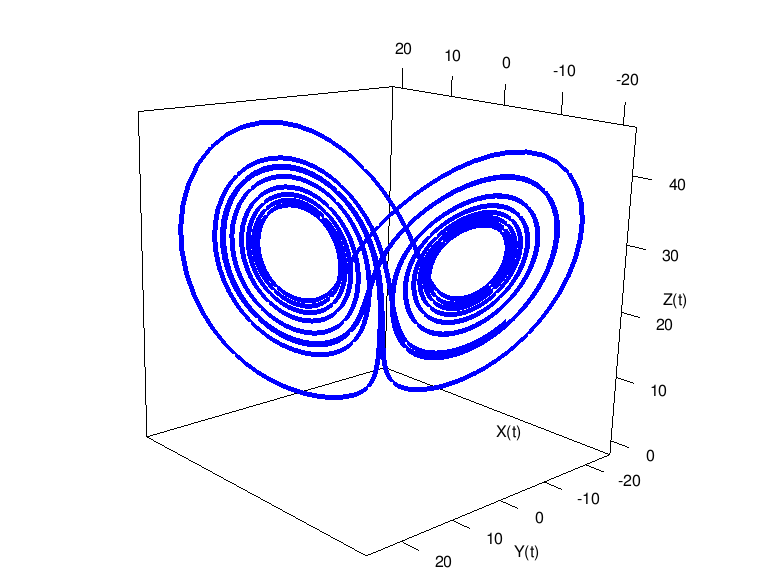
\includegraphics[scale=.25]{lorenzattractor}
  \caption{$\sigma=10$, $\rho=28$ and $\beta=3/8$}
       \end{figure}
     \end{column}
  \end{columns}
 \end{frame}


 
 %+++++++++++++++++++++++++++++++++++++++++++++++++++
\begin{frame}
\frametitle{Time-Delay Embedding Example }

\begin{figure}
 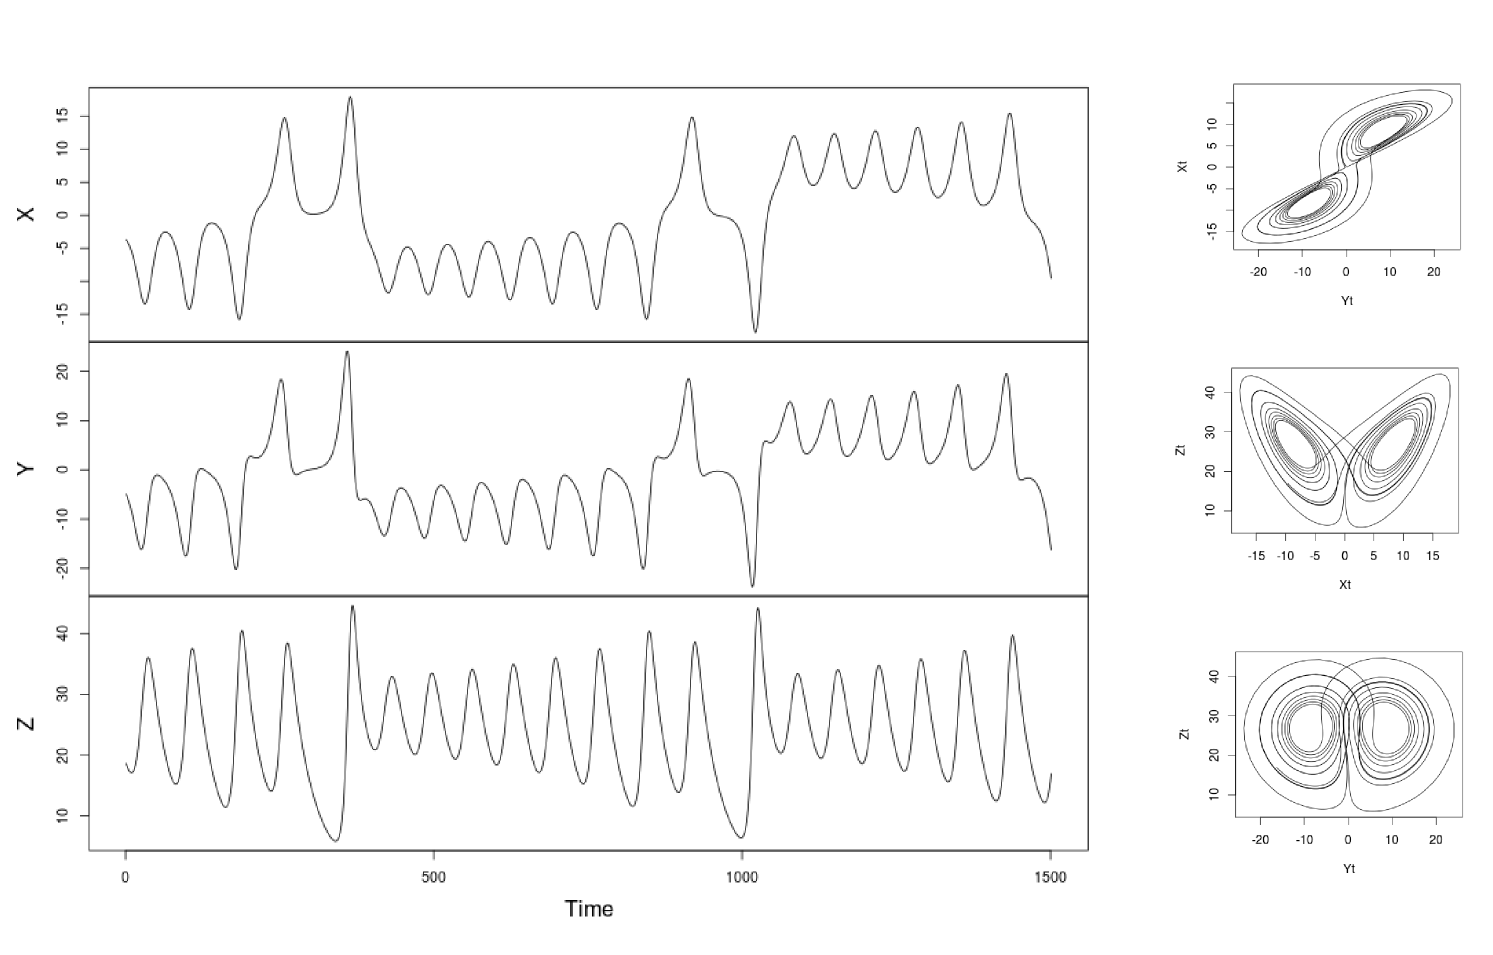
\includegraphics[scale=.2]{timeseries_2dmanifolds} \\
\caption{Time series of the Lorenz System and 2D manifolds}
\end{figure} 
 
\end{frame}




%+++++++++++++++++++++++++++++++++++++++++++++++++++
%%%%%%%%%%%%%%%
%%ANIMATION in evince
\begin{frame}
\frametitle{Time-Delay Embedding Example}
\vspace{-9mm}
\begin{columns}[onlytextwidth]
  \begin{column}{0.5\textwidth}
\begin{figure}
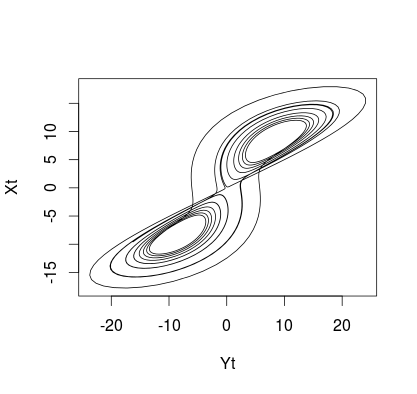
\includegraphics[scale=.3]{XY} 
\caption{Original Manifold}
\end{figure} 
\end{column} 

\begin{column}{0.5\textwidth}

\begin{figure}
\multiinclude[format=png,graphics={scale=0.25}]{images_frames_for_TAU/join} 
% \includegraphics[scale=0.3]{images_frames_for_TAU/manifold_d3_t-10}
\caption{Reconstructed Manifold}
\end{figure}
\end{column}
\end{columns}
\end{frame}










%+++++++++++++++++++++++++++++++++++++++++++++++++++
%+++++++++++++++++++++++++++++++++++++++++++++++++++
\section{Preliminary Experiments}

% %+++++++++++++++++++++++++++++++++++++++++++++++++++
% \begin{frame}
% \frametitle{My goals this month}
% 
% 
%    \begin{itemize}	
%       \item Determine the technique(s) to quantify the dexterity of 
%         Salsa Dancers based on the analysis of the reconstructed state space.
%       \item Submit a paper in The International Symposium on Wearable Computers (ISWC).
%         Deadline: April 10th, 2015.
%     \end{itemize}
% 
% 
% \end{frame}
% %---------------------------------------------------






%+++++++++++++++++++++++++++++++++++++++++++++++++++
\begin{frame}
\frametitle{}

\vspace{2cm}
% \begin{center}
% \LARGE{QUESTIONS?} 
% \end{center}

\vspace{1cm}

\normalsize 
\textbf{Miguel P. Xochicale} \\
Doctoral Researcher in Human-Robot Interaction \\
University of Birmingham, U.K. \\ 
{\color{blue} \href{http://mxochicale.github.io/}{http://mxochicale.github.io/ } } \\

   
\vspace{1cm}



\includegraphics[scale=.4]{CC4}
\tiny{ 
\textbf{My own pictures are release under CC BY-NC 4.0
{\color{blue} \href{http://creativecommons.org/licenses/by-nc/4.0/}{http://creativecommons.org/licenses/by-nc/4.0/} } \\
Give credits to: Miguel P. Xochicale
}
}

\end{frame}
%---------------------------------------------------




% 
% % Creates the cover page.
%  \frame{\titlepage}



\end{document}

